\documentclass{article}

\usepackage{graphicx}
\usepackage{subfig}
\usepackage{listings}

\begin{document}

\section{Week 1 (6/20/16 - 6/26/16)}
    \subsection{Tasks}
    \begin{itemize}
        \item Idea generation
        \item Early drafts
        \item Early game prototype
    \end{itemize}

    \subsection{Idea generation}
        Required constraints:
        \begin{itemize}
            \item Game
            \item Heartbeat or breathing sensor
            \item Physical computing
            \item Q-learning
            \item Affective computing or soma-aesthetics
        \end{itemize}

        \subsubsection{Final Concept: Flappy Penguin (working name)}
            After some brain storing we settled on a game in the spirit of \em Flappy Bird \em featuring:
            \begin{itemize}
                \item ``Protagonist'' is a penguin
                \item Side-scrolling movement
                \item Ice blocks entering the stage as obstacles
                \item \em Physical object \em controls penguin movement
                \item Breath-meter indicates penguins remaining breath
                \item User breathing while the penguin is under water reduces the breath-meter
                \item User breathing while the penguin is at the water surface replenishes breath-meter
                \item Empty breath meter means death by suffocation, i.e. game over
                \item Additional air bubbles can be collected under water to increase breath
                \item \em Q-learning \em used for either placement of air bubbles of a second, computer-controlled penguin
                \item Visually using the style of \em Thomas was Alone \em
            \end{itemize}

\clearpage

    \subsection{Early drafts}
        See Fig. \ref{fig:concepts}
        \begin{figure}[h]
            \subfloat[Sketches]{
                \includegraphics[width=0.45\textwidth]{img/01_sketches.png}
            }
            \qquad
            \subfloat[Mockup]{
                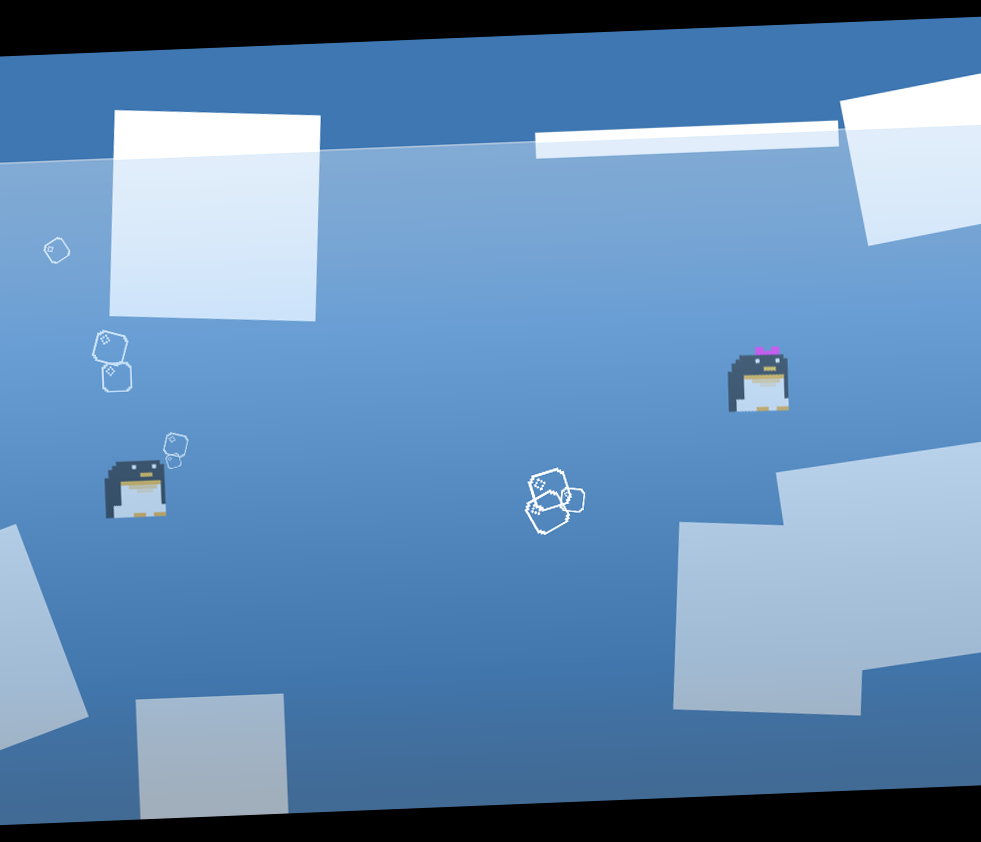
\includegraphics[width=0.45\textwidth]{img/02_mockup.png}
            }
            \caption{Concept}
            \label{fig:concepts}
        \end{figure}

\clearpage

    \subsection{Early game prototype}
        See Fig. \ref{fig:prototype_screenshots}
        \begin{figure}[h]
            % \subfloat[Early prototype]{
                % \includegraphics[width=0.45\textwidth]{img/03_prototype_screenshot.png}
            % }
            \subfloat[Early game assets]{
                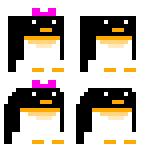
\includegraphics[width=0.45\textwidth]{img/04_penguin_assets.png}
            }
            \qquad
            \subfloat[Prototype using first few assets]{
                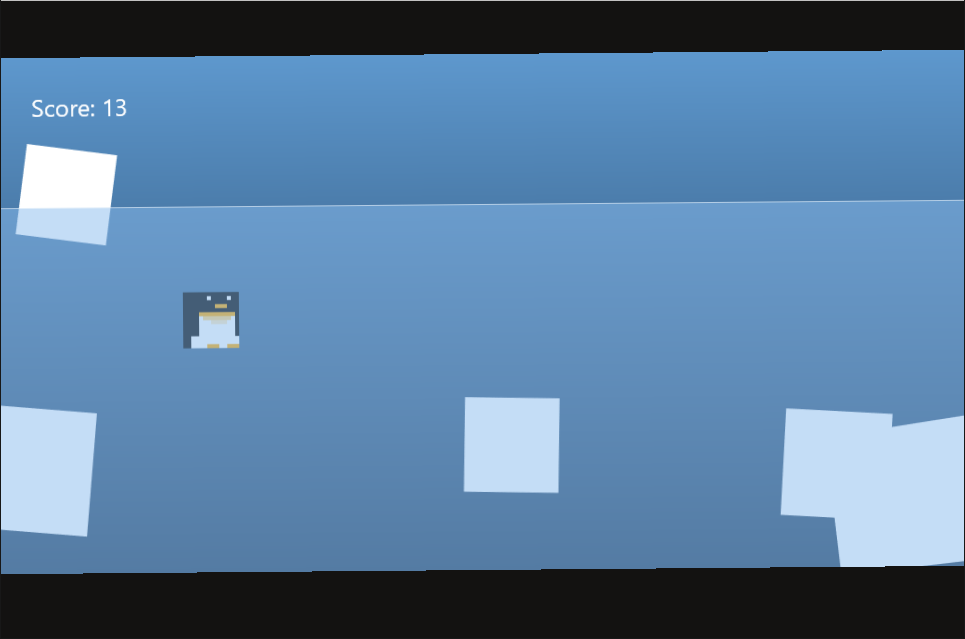
\includegraphics[width=0.45\textwidth]{img/05_prototype_screenshot.png}
            }
            \par
            \subfloat[Prototype using first few assets]{
                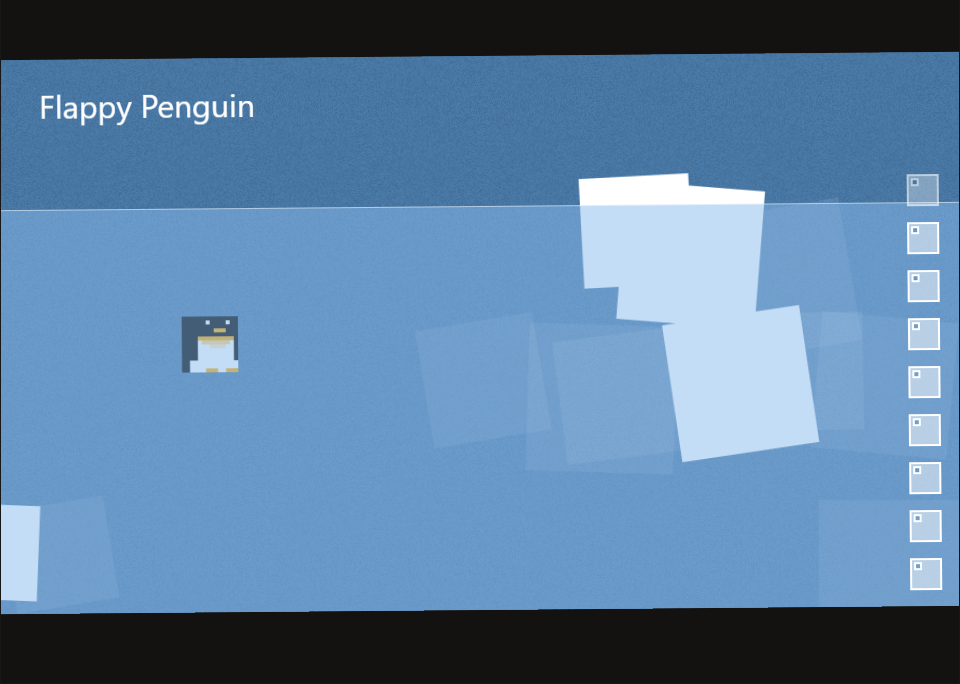
\includegraphics[width=0.45\textwidth]{img/06_prototype_screenshot.png}
            }
            \caption{Screenshots of different iterations}
            \label{fig:prototype_screenshots}
        \end{figure}

\section{Week 2 (6/27/16 - 7/3/16)}
    This weeks tasks:
    \begin{itemize}
        \item Incremental improvements of the game
        \item Breathing sensor integration
        \item Bend sensor integration
    \end{itemize}

    \subsection{Game improvements}
        By now the game includes the following components
        \begin{itemize}
            \item Basic scene layout
            \item Jumping by keyboard input
            \item Random obstacle generation
            \item Obstacle collision
            \item Breath and Breath GUI
            \item Pausing
        \end{itemize}

        Using a\em NodeJS\em server data is sent from the\em Arduino\em to the game via \em Socket.IO\em.

        With this we are now able to decrease the breath-meter when the user breathes while the penguin is beneath the water surface and increase it when it is above.

        \begin{figure}
            \centering
            \subfloat[Final game]{
                \includegraphics[width=0.45\textwidth]{img/09_final_game.png}
            }
            \qquad
            \subfloat[Victory screen]{
                \includegraphics[width=0.45\textwidth]{img/10_victory_screen.png}
            }
        \end{figure}

    \subsection{Integration of sensors}
        With the game being designed from scratch for sensor integration, moving data from Arduino to the web-page was very straight forward.

        We agreed on a simple JSON based protocol were messages had a type to distinguish between jumping and breathing input.

        We also distinguish between breathing in an out though it has no application in the game.

\section{Week 3 (7/4/16 - 7/10/16)}
    \subsection{Tasks}
    \begin{itemize}
        \item QLearning
    \end{itemize}

    \subsection{QLearning}
        Q-learning is used for a second penguin swimming away from the player penguin. This penguin swims at a steady pace unless it bumps into an ice-block. This will slow it down, allowing the chasing player penguin to catch up. The controls of this second penguin are learned with the goal of escaping the player.

        With a game such as Flappy Bird or Flappy Penguin, the state space is exceptionally large. In theory all obstacle positions, player position and in our version also opponent position and breath can factor into the full game state.

        We decided that for the way we train our second penguin, properly dodging obstacles, player position and breath were irrelevant. Furthermore only obstacles in front of the computer player were important to it.

        Thus we discretized the space in front of it into 16 sample points, for we encoded in binary whether there was an obstacle at this position or not.

        \begin{lstlisting}
        var state = 0;
        foreach (samplePoint) {
            if (obstacle at samplePoint) state = state | 1;
            state = state << 1
        }
        \end{lstlisting}

        We also had to include the position of the learning penguin for which we used some of the remaining 16 Bits.

        We discretized it to 64 values, 6 Bits, which we appended to the obstacle description.

        \begin{lstlisting}
        state = state << 6;
        state = state | discreetPenguinPosition;
        \end{lstlisting}

        Thus we were able to encode the state into a 22 Bits Integer. A state space of $2^22$ state is of course still exceptionally large, but in reality most states will never occur.

\section{Week 4 (11/7/15 - 18/7/16)}
    \subsection{Tasks}
    \begin{itemize}
        \item Fine tuning
        \item Presentation
    \end{itemize}
    \subsection{Fine tuning}
        The last few improvements to the game were:
        \begin{itemize}
            \item Adding air bubbles as visual cue when breathing under water.
            \item A shattering animation for ice-blocks when colliding with them
            \item Music integration
            \item Win and Game Over screens
        \end{itemize}

    \subsection{Presentation}
        The presentation section assigned to me was concerning q-learning.

        Since all listeners should have a solid understanding of how q-learning works and the vast majority being familiar with implementation details, only few parts of this topic were available as sufficiently interesting presentation subjects.

        The implementation details in JavaScript using the idiomatic way of callback functions and a second third runtime loop (aside from the rending and update loops) seemed not overly interesting, since they cover more JavaScript than q-learning.

        Thus we decided to cover one of the main challenges of q-learning during the presentation, the state description, which for a game as Flappy Penguin is highly non trivial.
        However, as previously discussion, we managed to encode the state into 22 Bits, thus producing a state space of size $\ll 2^22$.

        Unfortunately, shortly before the presentation our penguin-controller broke. We tried to quick-fix this by mapping the jump key on the presenter we used during the presentation. This way we still had a sort of physical controller and didn't need to resort to using the traditional way, the keyboard.

        What we did not anticipate was that another button on the presenter was by default mapped to the\em F5\em key, which, unfortunately, refreshed the page every time accidentally pressed.

        We did manage however to present and demo the functionality as well as the great trailer of game.

\end{document}
